\newpage
\hypertarget{emptyPartition tex}{}
\subsection{Implementing empty}
\texHeader

\begin{itemize}
 
\item[$\blacktriangleright$] To initialize your control flow, you can once again take advantage of eMolfon's type completion here. Inside the \texttt{empty}
declaration, press  \texttt{ctrl + space} and select \texttt{forEach} from the menu (Fig.~\ref{fig:typeCompletion}).

\vspace{1cm}

\begin{figure}[htpb]
\begin{center}
  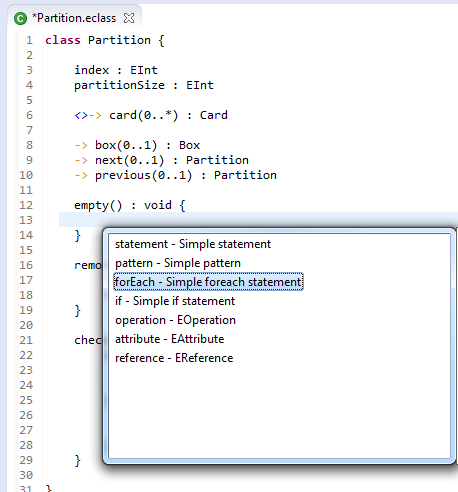
\includegraphics[width=0.7\textwidth]{eclipse_emptyTypeCompletion}
  \caption{eMoflon's Type Completion}
  \label{fig:typeCompletion}
\end{center}
\end{figure}

\vspace{1cm}

\item[$\blacktriangleright$] Create a single \texttt{deleteCardsInPartition}. Remove the suggested second pattern since you only need to complete the deletion
-- no extra steps required!

\item[$\blacktriangleright$] Your control flow should now resemble Fig.~\ref{fig:emptyControlFlow}.

\clearpage

\begin{figure}[htpb]
\begin{center}
  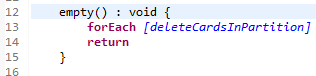
\includegraphics[width=0.5\textwidth]{eclipse_emptyControlFlow}
  \caption{Control flow for \texttt{empty}}
  \label{fig:emptyControlFlow}
\end{center}
\end{figure}

\item[$\blacktriangleright$] While similar to \texttt{removeCard}, this new pattern goes one step further by requesting a full destruction of card, instead of
just detaching the link. This means, in addition to destroying the link in \texttt{@this}, we need to set the binding operator for this variable to destroy. 
You can declare this special type by prefacing \texttt{card} with an `-~-' operator.

\vspace{0.5cm}

\item[$\blacktriangleright$] Your pattern should now resemble Fig.~\ref{fig:emptyPattern}.

\vspace{0.5cm}

\begin{figure}[htpb]
\begin{center}
  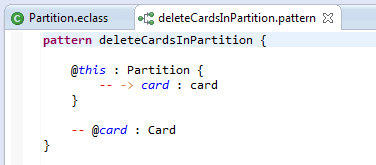
\includegraphics[width=0.6\textwidth]{eclipse_emptyPattern}
  \caption{Destroying an entire card}
  \label{fig:emptyPattern}
\end{center}
\end{figure}

\item[$\blacktriangleright$] That's it! Look at you go - you're just speeding through these SDMs now! To see how \texttt{empty} is done in the visual syntax,
review Fig.~\ref{fig:sdm_end} from the previous section.

\end{itemize}
